\documentclass{beamer}
\usepackage[dutch]{babel}
\usepackage{calc}
\usepackage[absolute,overlay]{textpos}
\usepackage{amsmath}
\usepackage{amsthm}
\usepackage{graphicx}
\usepackage{tikz}
\usetikzlibrary{decorations.pathreplacing}
\mode<presentation>{\usetheme{tud}}

\title[NedTrain Planner]{NedTrain Planner}
%\subtitle
\institute[TU Delft]{Construeren van Flexibele Roosters}
\author{Chris Bakker, Anton Bouter, Martijn den Hoedt}
\date{2 juli 2014}

\theoremstyle{definition}
\newtheorem{definitie}{Definitie}[section]

% Insert frame before each subsection (requires 2 latex runs)
\AtBeginSubsection[] {
	\begin{frame}<beamer>\frametitle{\titleSubsec}
		\tableofcontents[currentsection,currentsubsection]  % Generation of the Table of Contents
	\end{frame}
}
% Define the title of each inserted pre-subsection frame
\newcommand*\titleSubsec{Next Subsection}
% Define the title of the "Table of Contents" frame
\newcommand*\titleTOC{Outline}

% define a symbol which can be removed if you don't need it
\newcommand{\field}[1]{\mathbb{#1}}
\newcommand{\Zset}{\field{Z}}

\tikzset{
  invisible/.style={opacity=0},
  visible on/.style={alt={#1{}{invisible}}},
  alt/.code args={<#1>#2#3}{%
    \alt<#1>{\pgfkeysalso{#2}}{\pgfkeysalso{#3}} % \pgfkeysalso doesn't change the path
  },
}

\definecolor{darkyellow}{rgb}{0.7, 0.7, 0}
\definecolor{lightyellow}{rgb}{1.0, 1.0, 0}
\definecolor{darkgreen}{rgb}{0, 0.5, 0}
\definecolor{lightgreen}{rgb}{0, 0.7, 0}
\definecolor{darkcyan}{rgb}{0, 0.7, 0.7}
\definecolor{lightcyan}{rgb}{0, 1.0, 1.0}

\begin{document}

{
% remove the next line if you don't want a background image
\usebackgroundtemplate{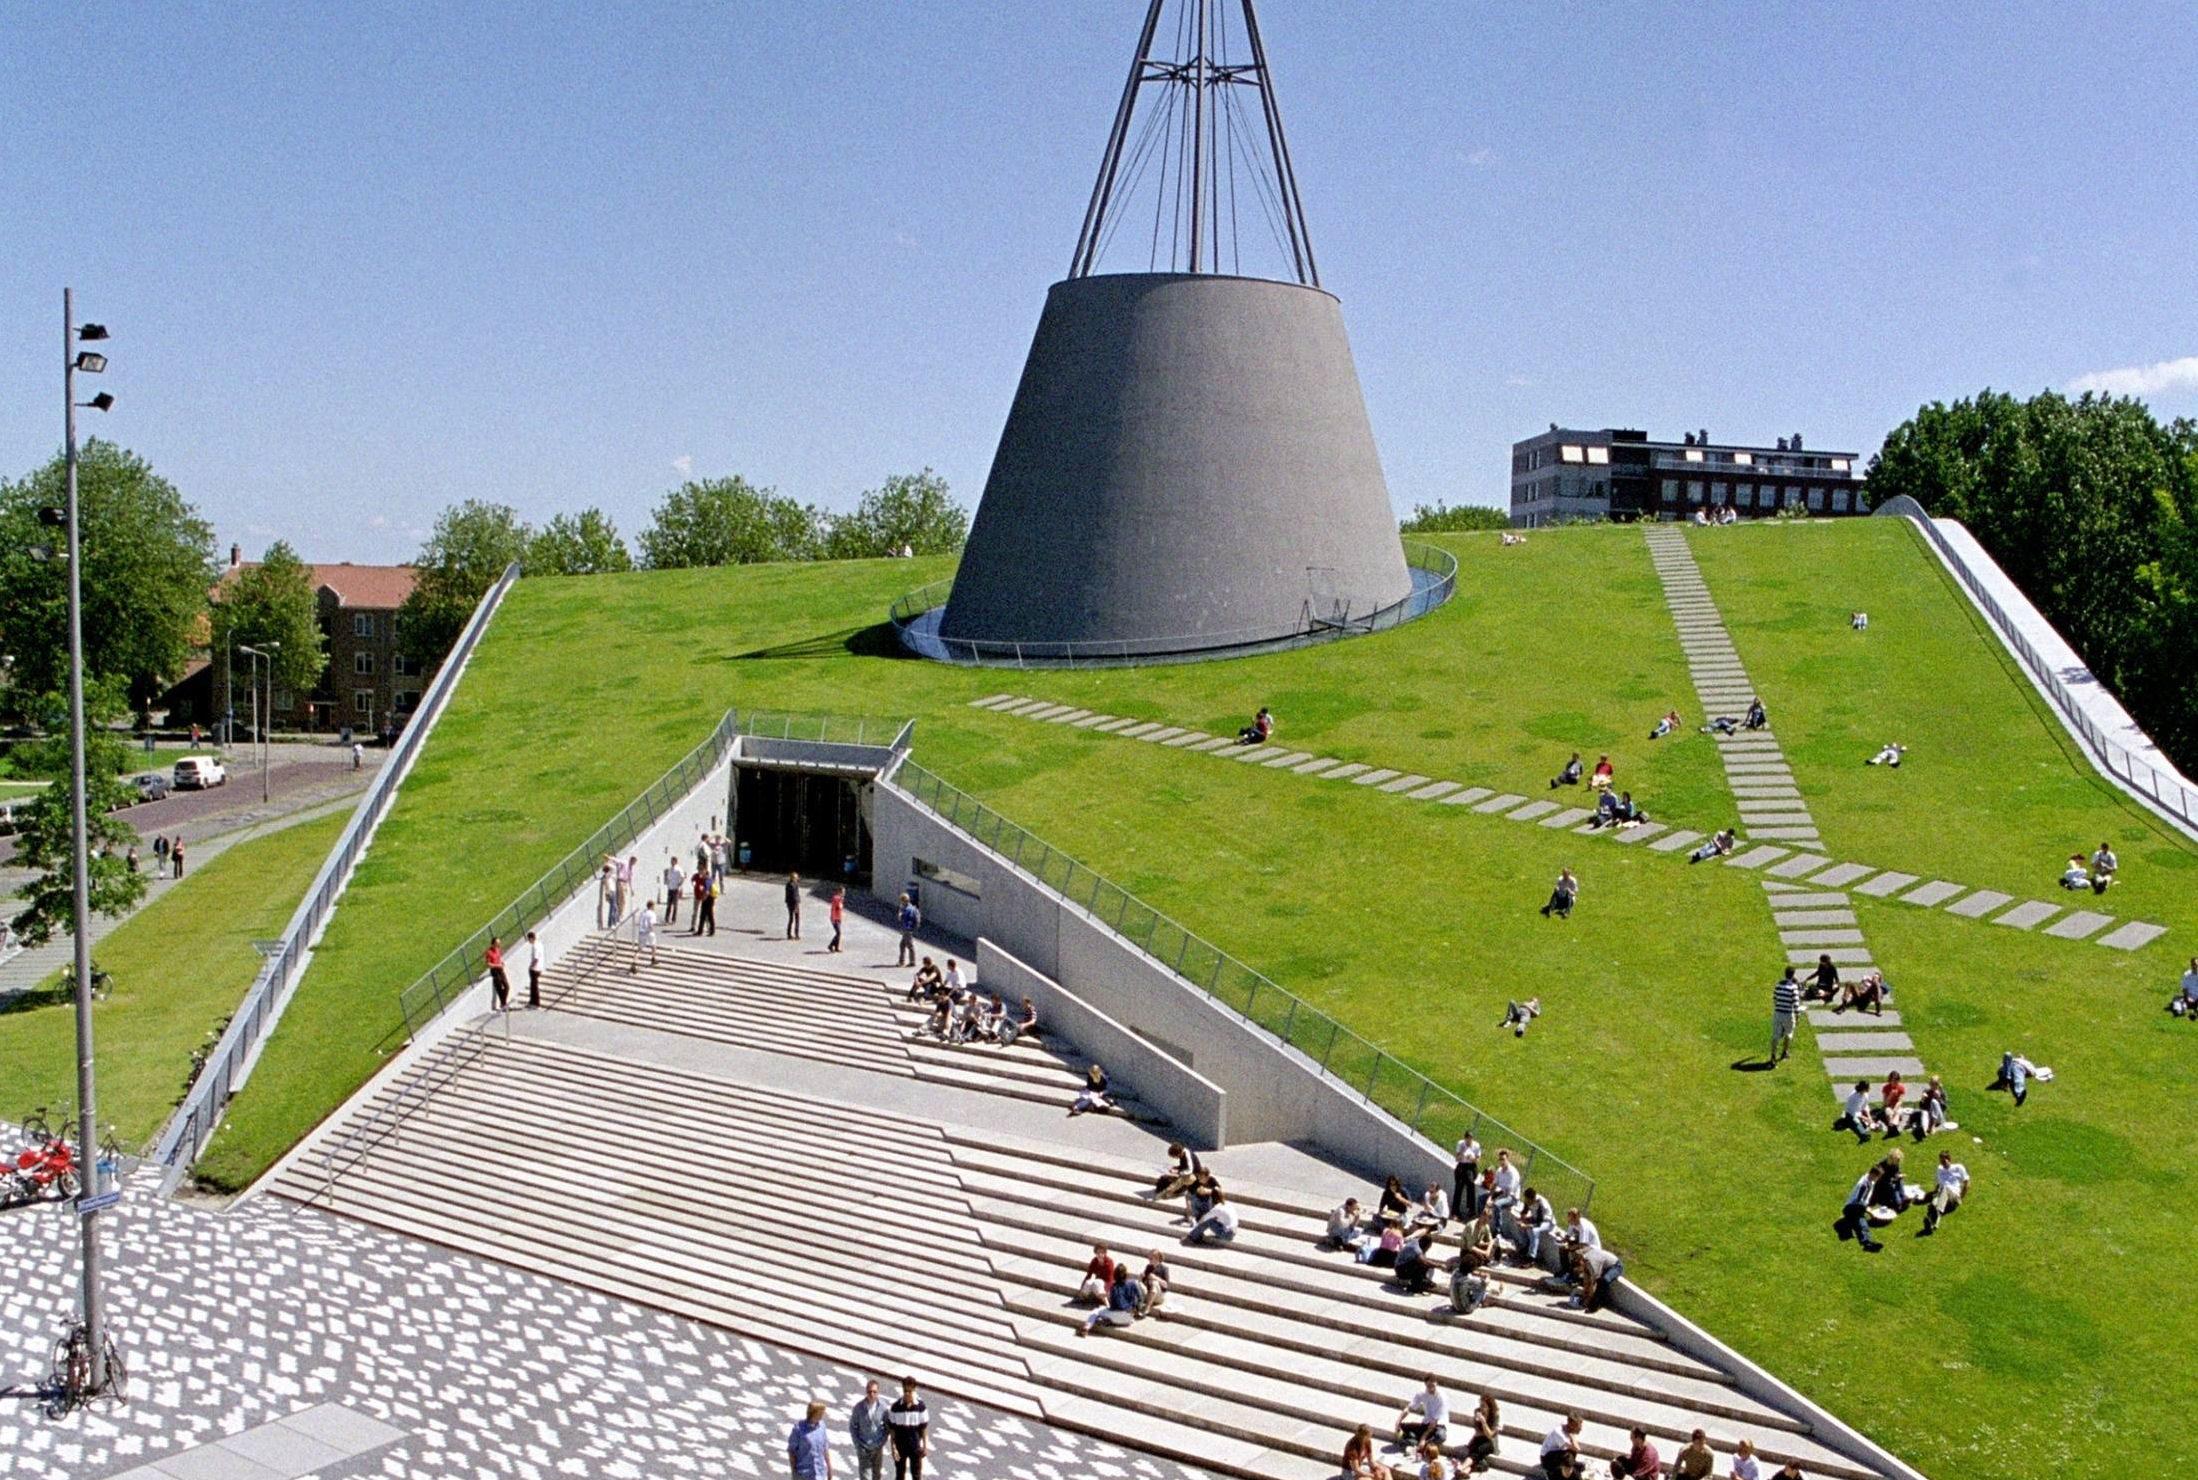
\includegraphics[width=\paperwidth,height=\paperheight]{images/background-titlepage.jpg}}%
\setbeamertemplate{footline}{\usebeamertemplate*{minimal footline}}
\frame{\titlepage}
}

\begin{frame}\frametitle{Inhoud}
    \begin{itemize}
        \item Opdrachtgevers
        \item Opdrachtomschrijving
        \begin{itemize}
        	\item Beschrijving Roosters
        	\item Voorbeeld Demo
        	\item Eisen van de Opdrachtgever
        \end{itemize}
        \item Aanpak en Hulpmiddelen
        \item Flexibiliteit
        \item Linear Programming
        \item Chaining Algoritme
        \item Andere Features
        \item Eind Demo
        \item Vragen
    \end{itemize}
\end{frame}

\begin{frame}\frametitle{Opdrachtgevers}
\begin{columns}[T] % align columns
    \begin{column}{.55\textwidth}
        \begin{itemize}
            \item NedTrain 
            \begin{itemize}
                \item Nederlandse Spoorwegen
                \item $250$ treinen op $30$ locaties
                \item $3500$ werknemers
                \item ir. Bob Huisman
            \end{itemize}
        \end{itemize}
        \vspace{1.8cm}
        \begin{itemize}
            \item TU Delft
            \begin{itemize}
                \item Algoritmiek groep
                \item prof. dr. Cees Witteveen
            \end{itemize}  
        \end{itemize}
    \end{column}%
    \begin{column}{.45\textwidth}
        
\includegraphics[width=4.5cm]{images/logo-nedtrain.jpg}
        \vspace{1cm}
        
\includegraphics[width=5cm]{images/tudelft_logo.pdf}
    \end{column}%
\end{columns}
\end{frame}


\begin{frame}\frametitle{Eigenschappen van roosters}
	\begin{columns}[T]
	    \begin{column}{.4\textwidth}
			\begin{itemize}
		        \item Activiteiten
		        \begin{itemize}
		            \item Stoelen vervangen
		            \item Graffiti verwijderen      
		        \end{itemize}
		        \item Resources
	            \begin{itemize}
	                \item Monteurs
	                \item Schoonmakers
	                \item Werkplaatsen
	            \end{itemize}
		    \end{itemize}
	    \end{column}
	    \begin{column}{.5\textwidth}
	    	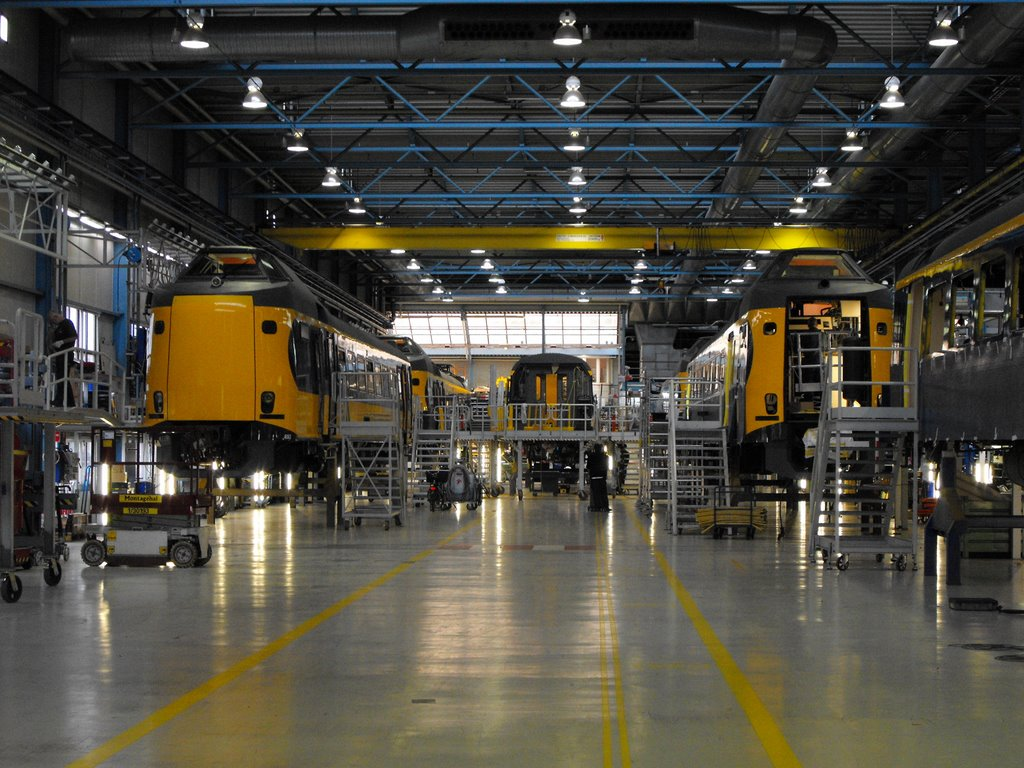
\includegraphics[width=4.5cm]{images/werkplaats.jpg}
	    \end{column}
  	\end{columns}
    \begin{itemize}
        \item Voorwaarden
        \begin{itemize}
        	\item Capaciteit resources
            \item Deadlines van activiteiten
            \item Voorrangsrelaties
        \end{itemize}
    \end{itemize}
\end{frame}

\begin{frame}\frametitle{NedTrain Planner}
	\begin{center}
		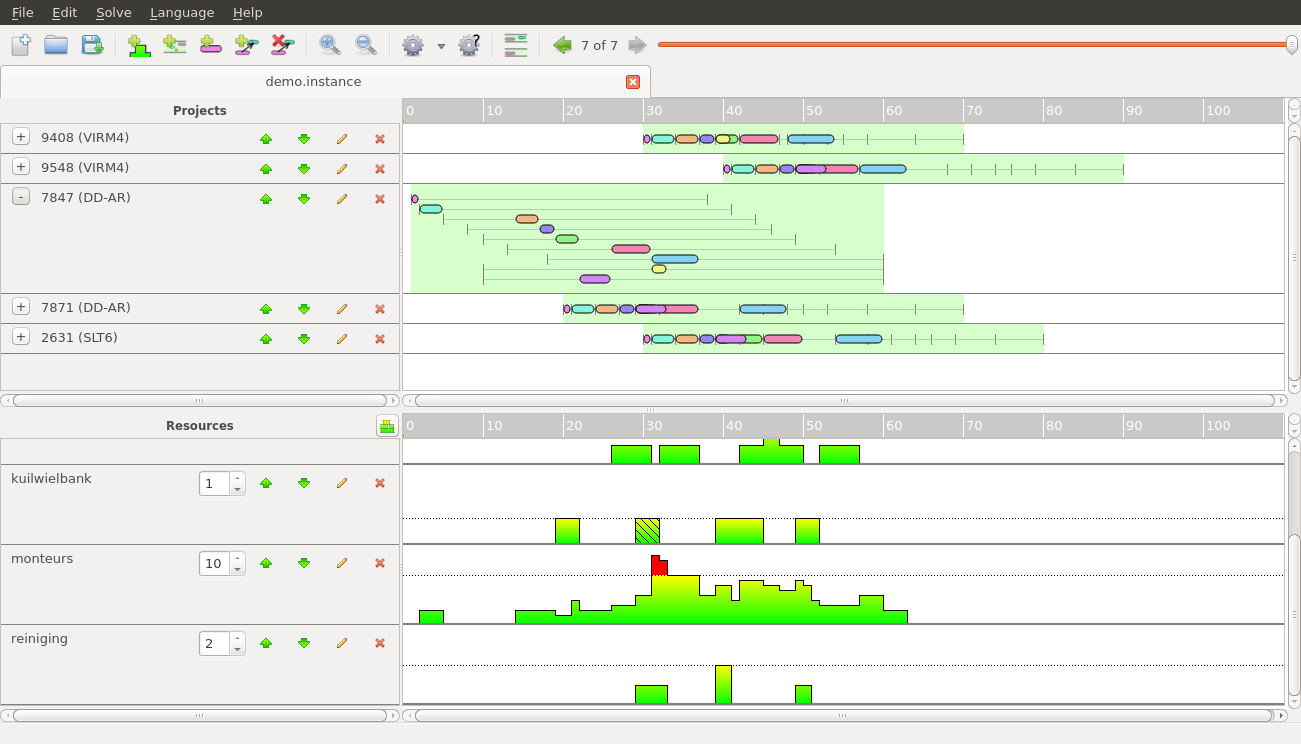
\includegraphics[width=11cm]{images/TMSconflictGUI.png}
	\end{center}
\end{frame}

\begin{frame}\frametitle{Opdrachtomschrijving}
	\begin{itemize}
		\item Functionele eisen
		\begin{itemize}
			\item De capaciteit van de resources mag niet overschreden worden bij het verschuiven van activiteiten
			\item De flexibiliteit van een rooster moet berekend worden
			\item De flexibiliteit van een rooster moet weergegeven en ge\"evalueerd kunnen worden
		\end{itemize}
		\item Niet-Functionele eisen
		\begin{itemize}
			\item De applicatie moet beschikbaar worden gemaakt voor Windows 7
			\item De applicatie moet makkelijk overdraagbaar zijn voor een volgend project
		\end{itemize}
	\end{itemize}
\end{frame}
\begin{frame}\frametitle{Aanpak en Hulpmiddelen}
	\begin{columns}[T]
  		\begin{column}{.7\textwidth}
			\begin{itemize}
				\item Scrum
					\begin{itemize}
						\item Software ontwikkelmethode
						\item Sprints van een week
					\end{itemize}
				\item Bitbucket
					\begin{itemize}
						\item Hosting website voor versiebeheersysteem
						\item Git
					\end{itemize}
				\item Qt
					\begin{itemize}
						\item Cross-platform applicatie framework
					\end{itemize}
				\item Google Test
					\begin{itemize}
						\item C++ Test Framework
					\end{itemize}
				\item Jenkins
					\begin{itemize}
						\item Continuous integration
					\end{itemize}
			\end{itemize}
		\end{column}
		\begin{column}{.3\textwidth}
			
\includegraphics[width=0.45\textwidth]{images/scrum.png}\\
			
\includegraphics[width=0.45\textwidth]{images/bitbucket.jpg}\\
			
\includegraphics[width=0.45\textwidth]{images/qt.jpg}\\
			
\includegraphics[width=0.45\textwidth]{images/jenkins.png}\\
		\end{column}
	\end{columns}
\end{frame}
\begin{frame}\frametitle{Flexibiliteit (1)}
    \begin{itemize}
        \item Hoe wordt flexibiliteit gemeten?
        \begin{itemize}
            \item<4-> Voor \'e\'en taak: $flex_t = t^+ - t^-$
        \end{itemize}
    \end{itemize}

    \newcommand{\widthpic}{100mm}
    \newcommand{\heightpic}{10mm}
    \newcommand{\offset}{2mm}
    \begin{tikzpicture}
        \coordinate (A) at (0, \heightpic /2);
        \coordinate (B) at (\widthpic, \heightpic /2);
        \coordinate (A1) at (0, 0);
        \coordinate (A2) at (0, \heightpic);
        \coordinate (B1) at (\widthpic, 0);
        \coordinate (B2) at (\widthpic, \heightpic);

        \draw [very thick] (A) -- (B);

        \filldraw[very thick, draw=darkgreen,fill=lightgreen, visible on=<1>] (10mm, \offset) rectangle (35mm, 8mm);
        \filldraw[very thick, draw=darkgreen,fill=lightgreen, visible on=<2>] (0mm, \offset) rectangle (25mm, 8mm);
        \filldraw[very thick, draw=darkgreen,fill=lightgreen, visible on=<3->] (75mm, \offset) rectangle (100mm, 8mm);

        \node[visible on=<2->] at (0mm,-3mm) {$t^-$};
        \node[visible on=<3->] at (75mm,-3mm) {$t^+$};

        \draw [very thick] (A1) -- (A2);
        \draw [very thick] (B1) -- (B2);
    \end{tikzpicture}
\end{frame}

\begin{frame}\frametitle{Flexibiliteit (2)}
    \begin{itemize}
        \item Hoe wordt flexibiliteit gemeten?
        \begin{itemize}
            \item Voor \'e\'en taak: $flex_t = t^+ - t^-$
            \item Voor hele schema: $flex_{totaal} = \sum_{t \in T}(t^+ - t^-)$    
            \item<2-> Voorrangsrelatie: $a \prec b$
        \end{itemize}
    \end{itemize}

    \newcommand{\widthpic}{100mm}
    \newcommand{\offset}{2mm}
    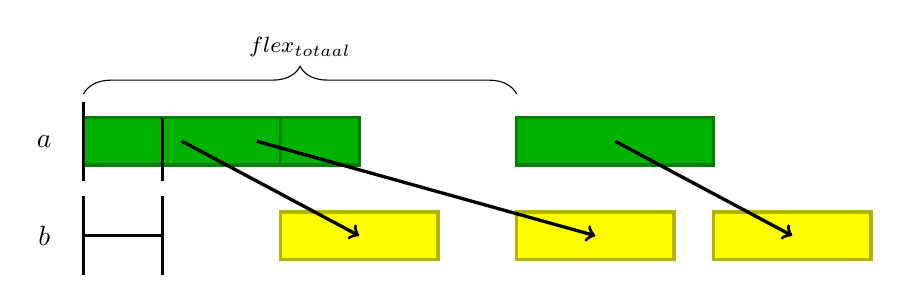
\begin{tikzpicture}
        \coordinate (A) at (0, 17mm);
        \coordinate (B) at (\widthpic, 17mm);
        \coordinate (A1) at (0, 12mm);
        \coordinate (A2) at (0, 22mm);
        \coordinate (B1) at (\widthpic, 12mm);
        \coordinate (B2) at (\widthpic, 20mm);

        \coordinate (C) at (0, 5mm);
        \coordinate (D) at (\widthpic, 5mm);
        \coordinate (C1) at (0, 0mm);
        \coordinate (C2) at (0, 10mm);
        \coordinate (D1) at (\widthpic, 0mm);
        \coordinate (D2) at (\widthpic, 10mm);

        \draw [very thick] (A) -- (B);
        \draw [very thick] (C) -- (D);

        \node at (-5mm,17mm) {$a$};
        \node at (-5mm,5mm) {$b$};

        % ergens in het midden
        \filldraw[very thick, draw=darkgreen,fill=lightgreen, visible on=<1-2>] (10mm, 14mm) rectangle (35mm, 20mm);
        \filldraw[very thick, draw=darkyellow,fill=lightyellow, visible on=<1-2>] (55mm, 2mm) rectangle (75mm, 8mm);

        % aan het begin
        \filldraw[very thick, draw=darkgreen,fill=lightgreen, visible on=<3>] (0mm, 14mm) rectangle (25mm, 20mm);
        \filldraw[very thick, draw=darkyellow,fill=lightyellow, visible on=<3>] (25mm, 2mm) rectangle (45mm, 8mm);

        % aan het einde
        \filldraw[very thick, draw=darkgreen,fill=lightgreen, visible on=<4->] (55mm, 14mm) rectangle (80mm, 20mm);
        \filldraw[very thick, draw=darkyellow,fill=lightyellow, visible on=<4->] (80mm, 2mm) rectangle (100mm, 8mm);
        
        % curly bracket
        \draw [decorate,decoration={brace,amplitude=10pt}, visible on=<5>]
        (0mm,23mm) -- (55mm,23mm) node [black,midway, yshift=6mm] 
        {\footnotesize $flex_{totaal}$};

        \draw [very thick] (A1) -- (A2);
        \draw [very thick] (B1) -- (B2);
        \draw [very thick] (C1) -- (C2);
        \draw [very thick] (D1) -- (D2);

        \draw [very thick, ->, visible on=<2>] (22mm, 17mm) -- (65mm, 5mm);
        \draw [very thick, ->, visible on=<3>] (12.5mm, 17mm) -- (35mm, 5mm);
        \draw [very thick, ->, visible on=<4->] (67.5mm, 17mm) -- (90mm, 5mm);
    \end{tikzpicture}
\end{frame}

\begin{frame}\frametitle{Flexibiliteit (3)}
    \begin{itemize}
        \item Voor hele schema: $flex_{totaal} = \sum_{t \in T}(t^+ - t^-)$
        \item Onafhankelijke intervallen
    \end{itemize}

    \newcommand{\widthpic}{100mm}
    \newcommand{\offset}{2mm}
    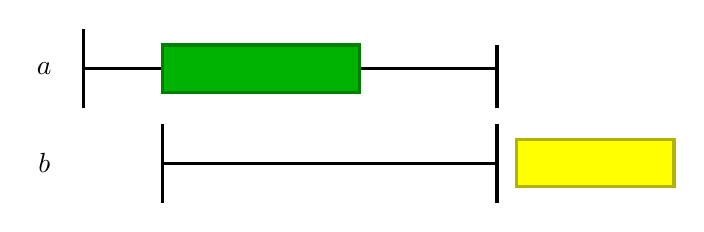
\begin{tikzpicture}
        \coordinate (A) at (0, 17mm);
        \coordinate (B) at (52.5mm, 17mm);
        \coordinate (A1) at (0, 12mm);
        \coordinate (A2) at (0, 22mm);
        \coordinate (B1) at (52.5mm, 12mm);
        \coordinate (B2) at (52.5mm, 20mm);

        \coordinate (C) at (52.5mm, 5mm);
        \coordinate (D) at (\widthpic, 5mm);
        \coordinate (C1) at (52.5mm, 0mm);
        \coordinate (C2) at (52.5mm, 10mm);
        \coordinate (D1) at (\widthpic, 0mm);
        \coordinate (D2) at (\widthpic, 10mm);

        \draw [very thick] (A) -- (B);
        \draw [very thick] (C) -- (D);

        \node at (-5mm,17mm) {$a$};
        \node at (-5mm,5mm) {$b$};

        % ergens in het midden
        \filldraw[very thick, draw=darkgreen,fill=lightgreen] (10mm, 14mm) rectangle (35mm, 20mm);
        \filldraw[very thick, draw=darkyellow,fill=lightyellow] (55mm, 2mm) rectangle (75mm, 8mm);
        
        \draw [very thick] (A1) -- (A2);
        \draw [very thick] (B1) -- (B2);
        \draw [very thick] (C1) -- (C2);
        \draw [very thick] (D1) -- (D2);
    \end{tikzpicture}
\end{frame}

\begin{frame}\frametitle{Linear Programming}
    \begin{definitie}
        \begin{align}
            \text{max:}& \quad \sum_{t \in T} (t^+ - t^-) & \nonumber \\
            % constraint 1
            \only<1>{\phantom{\text{met voorwaarden:}} & \phantom{\quad t^- \leq t^+} & \phantom{\forall t \in T} \nonumber \\}
            \only<2->{\text{met voorwaarden:} & \quad t^- \leq t^+ & \forall t \in T \nonumber \\} 
            % contraint 2
            \only<-2>{& \phantom{\quad a^+ - b^- \leq -d_a} & \phantom{\forall (a \prec b) \in C} \nonumber}
            \only<3-8>{& \phantom{\quad a^+ - b^- \leq -d_a} & \forall (a \prec b) \in C \nonumber}
            \only<9->{& \quad a^+ + d_a \leq b^- & \forall (a \prec b) \in C \nonumber}
        \end{align}
    \end{definitie}

    \begin{itemize}
        \item \only<4->{$a \prec b$} \only<8->{$\quad \Rightarrow \quad a^+ + d_a \leq b^-$}
        \item<10-> COIN-OR Linear Programming Solver (CLP)
    \end{itemize}

    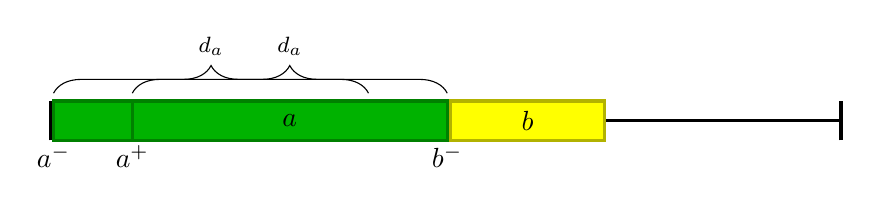
\begin{tikzpicture}
        \draw[very thick, visible on=<4->] (-0.4mm, 2.5mm) -- (100mm, 2.5mm);
        \draw[very thick, visible on=<4->] (-0.4mm, 0mm) -- (-0.4mm, 5mm);
        \draw[very thick, visible on=<4->] (100mm, 0mm) -- (100mm, 5mm);

        \filldraw[very thick, draw=darkgreen,fill=lightgreen, visible on=<4-5>] (0mm,0mm) rectangle (40mm,5mm) node[pos=.5] {$a$};
        \filldraw[very thick, draw=darkgreen,fill=lightgreen, visible on=<6->] (10mm,0mm) rectangle (50mm,5mm) node[pos=.5] {$a$};
        \filldraw[very thick, draw=darkyellow,fill=lightyellow, visible on=<4->] (50.4mm,0mm) rectangle (70mm,5mm) node[pos=.5] {$b$};

        \draw [decorate, decoration={brace,amplitude=10pt}, visible on=<5>]
        (0mm,6mm) -- (40mm,6mm) node [black,midway, yshift=6mm] 
        {\footnotesize $d_a$};
\draw [decorate, decoration={brace,amplitude=10pt}, visible on=<6->]
        (10mm,6mm) -- (50mm,6mm) node [black,midway, yshift=6mm] 
        {\footnotesize $d_a$};

        \node[visible on=<5->] at (0mm, -2mm) {$a^-$};
        \node[visible on=<7->] at (10mm, -2mm) {$a^+$};
        \node[visible on=<5->] at (50mm, -2mm) {$b^-$};
    \end{tikzpicture}
\end{frame}

\begin{frame}[fragile]\frametitle{Chaining (1)}
    \begin{itemize}      
        \item Resource conflicten oplossen
        %\item<8-> $a \prec b$
    \end{itemize}
    \vspace{5mm}
    \newcommand{\widthpic}{100mm}
    \newcommand{\heightpic}{30mm}
    \newcommand\dashline[1]{\draw[thick, dashed] (0, #1) -- (100mm, #1)}
    \newcommand\normline[1]{\draw[very thick] (0, #1) -- (100mm, #1)}
    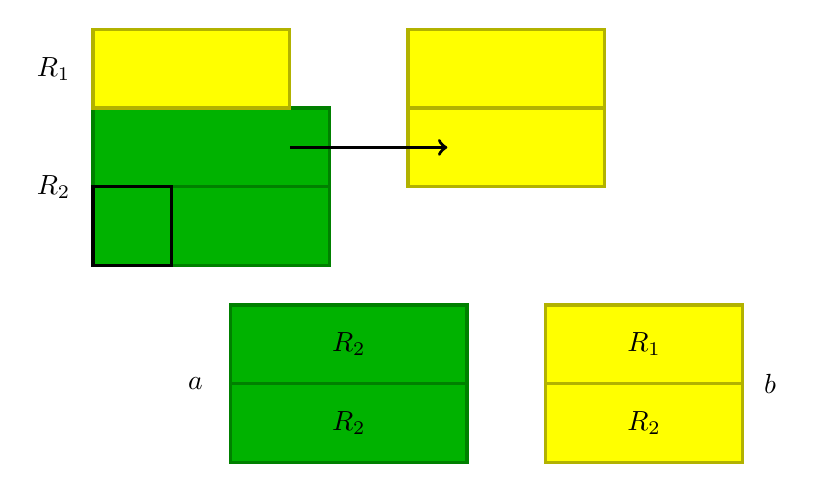
\begin{tikzpicture}
        \coordinate (A) at (0, 0);
        \coordinate (B) at (\widthpic, 0);
        \coordinate (C) at (\widthpic, \heightpic);
        \coordinate (D) at (0, \heightpic);

        % onder de resources
        % taak A
        \filldraw[very thick, draw=darkgreen,fill=lightgreen, visible on=<2-3>] (17.5mm, -15mm) rectangle (47.5mm, -5mm) node[pos=.5] {$R_2$};
        \filldraw[very thick, draw=darkgreen,fill=lightgreen, visible on=<2-4>] (17.5mm, -25mm) rectangle (47.5mm, -15mm) node[pos=.5] {$R_2$};
        \node[visible on=<2-4>] at (13mm,-15mm) {$a$};

        % taak B
        \filldraw[very thick, draw=darkyellow,fill=lightyellow, visible on=<3-5>] (57.5mm, -15mm) rectangle (82.5mm, -5mm) node[pos=.5] {$R_1$};
        \filldraw[very thick, draw=darkyellow,fill=lightyellow, visible on=<3-6>] (57.5mm, -25mm) rectangle (82.5mm, -15mm) node[pos=.5] {$R_2$};
        \node[visible on=<3-6>] at (86mm,-15mm) {$b$};
            
        % geplaatst
        % taak A
        \filldraw[very thick, draw=darkgreen,fill=lightgreen, visible on=<4->] (0mm, 10mm) rectangle (30mm, 20mm);
        \filldraw[very thick, draw=darkgreen,fill=lightgreen, visible on=<5->] (0mm, 0mm) rectangle (30mm, 10mm);

        % taak B
        \filldraw[very thick, draw=darkyellow,fill=lightyellow, visible on=<6>] (0mm, 20mm) rectangle (25mm, 30mm);
        \filldraw[very thick, draw=darkyellow,fill=lightyellow, visible on=<7->] (40mm, 20mm) rectangle (65mm, 30mm);
        \filldraw[very thick, draw=darkyellow,fill=lightyellow, visible on=<7->] (40mm, 10mm) rectangle (65mm, 20mm);

        \draw[very thick] (A) rectangle (C);

        \dashline{1 * \heightpic / 3};
        \normline{2 * \heightpic / 3};

        \node at (-5mm, 25mm) {$R_1$};
        \node at (-5mm, 10mm) {$R_2$};
        
        \draw [->, very thick, visible on=<8->] (25mm, 15mm) -- (45mm, 15mm);
    \end{tikzpicture}
\end{frame}

\begin{frame}[fragile]\frametitle{Chaining (1)}
	\addtocounter{framenumber}{-1}
    \begin{itemize}      
        \item Resource conflicten oplossen
    \end{itemize}
    \vspace{5mm}
    \newcommand{\widthpic}{100mm}
    \newcommand{\heightpic}{30mm}
    \newcommand\dashline[1]{\draw[thick, dashed] (0, #1) -- (100mm, #1)}
    \newcommand\normline[1]{\draw[very thick] (0, #1) -- (100mm, #1)}
    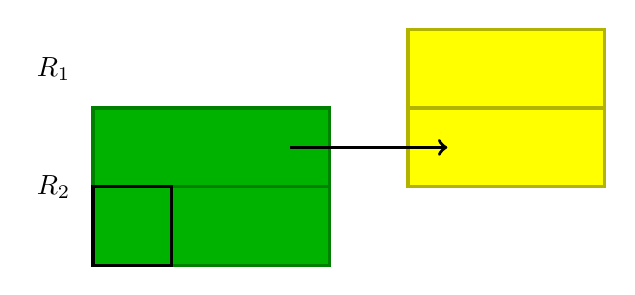
\begin{tikzpicture}
        \coordinate (A) at (0, 0);
        \coordinate (B) at (\widthpic, 0);
        \coordinate (C) at (\widthpic, \heightpic);
        \coordinate (D) at (0, \heightpic);
            
        % geplaatst
        % taak A
        \filldraw[very thick, draw=darkgreen,fill=lightgreen] (0mm, 10mm) rectangle (30mm, 20mm);
        \filldraw[very thick, draw=darkgreen,fill=lightgreen] (0mm, 0mm) rectangle (30mm, 10mm);

        % taak B
        \filldraw[very thick, draw=darkyellow,fill=lightyellow] (40mm, 20mm) rectangle (65mm, 30mm);
        \filldraw[very thick, draw=darkyellow,fill=lightyellow] (40mm, 10mm) rectangle (65mm, 20mm);

        \draw[very thick] (A) rectangle (C);

        \dashline{1 * \heightpic / 3};
        \normline{2 * \heightpic / 3};

        \node at (-5mm, 25mm) {$R_1$};
        \node at (-5mm, 10mm) {$R_2$};
        
        \draw [->, very thick] (25mm, 15mm) -- (45mm, 15mm);
    \end{tikzpicture}
    
    \begin{itemize}
    		\item $a \prec b$
    \end{itemize}
    
    \vspace{16mm}
\end{frame}
	
\begin{frame}[fragile] \frametitle{Chaining (2)}
    \newcommand{\widthpic}{100mm}
    \newcommand{\heightpic}{30mm}
    \newcommand\dashline[1]{\draw[thick, dashed] (0, #1) -- (100mm, #1)}
    \newcommand\normline[1]{\draw[very thick] (0, #1) -- (100mm, #1)}
    
	\begin{itemize}
		\item Minimaliseren van het aantal constraints.
	\end{itemize}
	\vspace{5mm}
    
	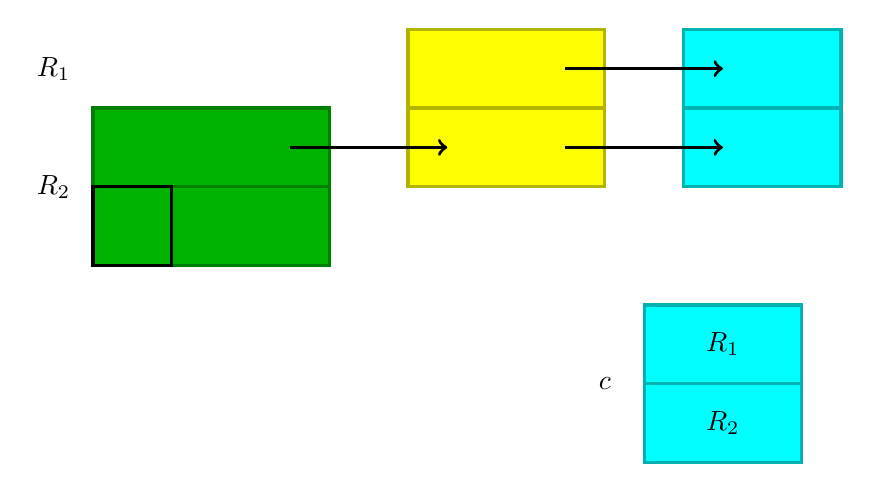
\begin{tikzpicture}
        \coordinate (A) at (0, 0);
        \coordinate (B) at (\widthpic, 0);
        \coordinate (C) at (\widthpic, \heightpic);
        \coordinate (D) at (0, \heightpic);
            
        % geplaatst
        % taak A
        \filldraw[very thick, draw=darkgreen,fill=lightgreen] (0mm, 10mm) rectangle (30mm, 20mm);
        \filldraw[very thick, draw=darkgreen,fill=lightgreen] (0mm, 0mm) rectangle (30mm, 10mm);

        % taak B
        \filldraw[very thick, draw=darkyellow,fill=lightyellow] (40mm, 20mm) rectangle (65mm, 30mm);
        \filldraw[very thick, draw=darkyellow,fill=lightyellow] (40mm, 10mm) rectangle (65mm, 20mm);
        
        % niet geplaatst
        % taak C
        \filldraw[very thick, draw=darkcyan,fill=lightcyan, visible on=<1>] (70mm, -15mm) rectangle (90mm, -5mm) node[pos=.5] {$R_1$};
        \filldraw[very thick, draw=darkcyan,fill=lightcyan, visible on=<1-3>] (70mm, -25mm) rectangle (90mm, -15mm) node[pos=.5] {$R_2$};
        \node[visible on=<1-3>] at (65mm,-15mm) {$c$};
        
        % wel geplaatst
        % taak C
        \filldraw[very thick, draw=darkcyan,fill=lightcyan, visible on=<2->] (75mm, 20mm) rectangle (95mm, 30mm);
        \filldraw[very thick, draw=darkcyan,fill=lightcyan, visible on=<4->] (75mm, 10mm) rectangle (95mm, 20mm);

        \draw[very thick] (A) rectangle (C);

        \dashline{1 * \heightpic / 3};
        \normline{2 * \heightpic / 3};

        \node at (-5mm, 25mm) {$R_1$};
        \node at (-5mm, 10mm) {$R_2$};
        
        \draw [->, very thick, visible on=<3->] (60mm, 25mm) -- (80mm, 25mm);
        \draw [->, very thick, visible on=<5->] (60mm, 15mm) -- (80mm, 15mm);
        \draw [->, very thick] (25mm, 15mm) -- (45mm, 15mm);
        %\draw [->, very thick, visible on=<2>] (60mm, 15mm) -- (70mm, -15mm);
    \end{tikzpicture}
\end{frame}

\begin{frame}\frametitle{Opgeleverde Producten}
\begin{itemize}
	\item Chaining algoritme en flexibiliteit
	\begin{itemize}
		\item Flexibiliteitsintervallen
		\item Een nieuwe resource profile view
		\item Solver stappen van chaining algoritme
	\end{itemize}
	
	\item Informatie en resultaten
	\begin{itemize}
		\item Flexibiliteitsmaten
		\item Veranderingen bij het opnieuw oplossen
		\item Tijdsduur en procentueel aandeel algoritmes
	\end{itemize}
	
	\item Overige
	\begin{itemize}
		\item Werkt onder Windows en Linux systemen
		\item Ge\"upgraded naar nieuwe versie Qt
		\item Gebruiksgemak verbeterd
		\item Code schoongemaakt en gerefactord
	\end{itemize}
\end{itemize}
\end{frame}

\begin{frame}\frametitle{Demo}
    \huge{\hfill Tijd voor een demo! \hfill}
\end{frame}

\begin{frame}\frametitle{Software Improvement Group}
    \hfill
    \begin{tikzpicture}[overlay]
        \node at (-2,0) {
\includegraphics[width=3cm]{images/sig.png}};
        
    \end{tikzpicture}
    \begin{itemize}
        \item 1$^e$ meting:
        \begin{itemize}
            \item "bijna 4 sterren"
            \item "lagere score voor Module Coupling, Unit Size en Unit Complexity"
        \end{itemize}
        \item 2$^e$ meting:
            \begin{itemize}
                \item "score voor onderhoudbaarheid ongeveer gelijk"
                \item "deelscore voor Unit Size van 3 naar 4 sterren is gestegen"
                \item bij Module Coupling weinig verbetering
                \item ''aanbevelingen van de vorige evaluatie zijn grotendeels meegenomen"
            \end{itemize}
    \end{itemize}
\end{frame}

\section{Conclusie}
Achteraf gezien kunnen we een aantal conclusies trekken over dit project. In het Plan van Aanpak wordt een aantal op te leveren features genoemd, onderverdeeld in drie categori\"en van prioriteit. Alle taken met hoge prioriteit zijn volbracht en in de categorie met taken van gemiddelde prioriteit stond de undo-functionaliteit, die wij niet hebben kunnen implementeren door een gebrek aan tijd. We hebben onderzocht wat er nodig zou om deze functionaliteit te \"implementeren en kwamen tot de conlusie dat dit erg veel tijd zou gaan kosten en niet in verhouding zou staan met wat het zou opleveren. In de categorie lage prioriteit hebben we alles kunnen doen, behalve \emph{"Het verduidelijken van het vergelijken van verschillende oplossingen."} We zijn erg tevreden nu we kunnen concluderen dat we zoveel features hebben kunnen maken.

We hebben allen veel geleerd van de programmeertaal \cpp\ en het Qt framework. Deze waren beide voor ons erg onbekend en vooral \cpp\ leverde soms aardig wat hobbels op in de weg naar succes. 

De samenwerking liep gesmeerd, dit mede doordat wij ook al aan een eerder project hebben samengewerkt. De feedback van onze begeleiders heeft ook zeker bijgedragen aan een beter eindproduct. Het feit dat andere groepen al aan dit project hebben gewerkt en zeer waarschijnlijk ook wij opgevolgd zullen worden door enthousiaste informatici maakt dit project realistischer dan elk ander project tijdens de bacheloropleiding. Wij vonden dit allen een zeer leerzaam en geslaagd Bachelorproject.

\begin{frame}\frametitle{Vragen}
    {\hfill%
    
\begin{tikzpicture}[thick,scale=5, every node/.style={transform shape}]
        \node at (0,0.7) {\Huge{Q}};
        \node at (0.45,0.9) {\huge{\&}};
        \node at (0.32,0.35) {\Huge{A}};
    \end{tikzpicture}%
    \hfill%
    }
\end{frame}


\end{document}
